%%%%%%%%%%%%%%%%%%%%%%%%%%%%%%%%%%%%%%%%%
% Beamer Presentation
% LaTeX Template
% Version 1.0 (10/11/12)
%
% This template has been downloaded from:
% http://www.LaTeXTemplates.com
%
% License:
% CC BY-NC-SA 3.0 (http://creativecommons.org/licenses/by-nc-sa/3.0/)
%
%%%%%%%%%%%%%%%%%%%%%%%%%%%%%%%%%%%%%%%%%

%----------------------------------------------------------------------------------------
%	PACKAGES AND THEMES
%----------------------------------------------------------------------------------------

\documentclass{beamer}

\mode<presentation> {

% The Beamer class comes with a number of default slide themes
% which change the colors and layouts of slides. Below this is a list
% of all the themes, uncomment each in turn to see what they look like.

%\usetheme{default}
%\usetheme{AnnArbor}
%\usetheme{Antibes}
%\usetheme{Bergen}
%\usetheme{Berkeley}
%\usetheme{Berlin}
%\usetheme{Boadilla}
%\usetheme{CambridgeUS}
%\usetheme{Copenhagen}
%\usetheme{Darmstadt}
%\usetheme{Dresden}
%\usetheme{Frankfurt}
%\usetheme{Goettingen}
%\usetheme{Hannover}
%\usetheme{Ilmenau}
%\usetheme{JuanLesPins}
%\usetheme{Luebeck}
\usetheme{Madrid}
%\usetheme{Malmoe}
%\usetheme{Marburg}
%\usetheme{Montpellier}
%\usetheme{PaloAlto}
%\usetheme{Pittsburgh}
%\usetheme{Rochester}
%\usetheme{Singapore}
%\usetheme{Szeged}
%\usetheme{Warsaw}

% As well as themes, the Beamer class has a number of color themes
% for any slide theme. Uncomment each of these in turn to see how it
% changes the colors of your current slide theme.

%\usecolortheme{albatross}
%\usecolortheme{beaver}
%\usecolortheme{beetle}
%\usecolortheme{crane}
%\usecolortheme{dolphin}
%\usecolortheme{dove}
%\usecolortheme{fly}
%\usecolortheme{lily}
%\usecolortheme{orchid}
%\usecolortheme{rose}
%\usecolortheme{seagull}
%\usecolortheme{seahorse}
%\usecolortheme{whale}
%\usecolortheme{wolverine}

%\setbeamertemplate{footline} % To remove the footer line in all slides uncomment this line
%\setbeamertemplate{footline}[page number] % To replace the footer line in all slides with a simple slide count uncomment this line

%\setbeamertemplate{navigation symbols}{} % To remove the navigation symbols from the bottom of all slides uncomment this line
}

\usepackage{hyperref}
\usepackage{verbatim}
\usepackage{graphicx} % Allows including images
\usepackage{booktabs} % Allows the use of \toprule, \midrule and \bottomrule in tables

%----------------------------------------------------------------------------------------
%	TITLE PAGE
%----------------------------------------------------------------------------------------

\title[ML: MKL]{Machine Learning: Multiple Kernel Learning} % The short title appears at the bottom of every slide, the full title is only on the title page

\author{Gustavo Ramirez} % Your name
%\institute[UCLA] % Your institution as it will appear on the bottom of every slide, may be shorthand to save space
%{
%University of California \\ % Your institution for the title page
%\medskip
%\textit{john@smith.com} % Your email address
%}
\date{\today} % Date, can be changed to a custom date

\begin{document}

\begin{frame}
\titlepage % Print the title page as the first slide
\end{frame}

\begin{frame}
\frametitle{Overview} % Table of contents slide, comment this block out to remove it
\tableofcontents % Throughout your presentation, if you choose to use \section{} and \subsection{} commands, these will automatically be printed on this slide as an overview of your presentation
\end{frame}

%----------------------------------------------------------------------------------------
%	PRESENTATION SLIDES
%----------------------------------------------------------------------------------------

%------------------------------------------------
%\section{First Section} % Sections can be created in order to organize your presentation into discrete blocks, all sections and subsections are automatically printed in the table of contents as an overview of the talk
%------------------------------------------------

%\subsection{Subsection Example} % A subsection can be created just before a set of slides with a common theme to further break down your presentation into chunks


\section{Brief Introduction to Machine Learning}

%------------------------------------------------

\begin{frame}
\frametitle{What exactly is Machine Learning?}

A lot of things.. and the field is constantly expanding.

\end{frame}

\begin{frame}
\frametitle{What exactly is Machine Learning?}

\textit{"[Machine Learning is the] field of study that gives computers the ability to learn without being explicitly programmed"}

\ \\

First step towards AI...

\ \\

Arthur Lee Samuel (1901-1990): computer gaming, artificial intelligence, machine learning, TeX, ...

\end{frame}


\begin{frame}
\frametitle{What exactly is Machine Learning?}

\textit{"A computer program is said to learn from experience E with respect to some task T and some performance measure P, if its performance on T, as measured by P, improves with experience E."}

\ \\

Tom Mitchell, Carnegie Mellon University

\end{frame}


\begin{comment}
\begin{frame}
\frametitle{What exactly is Machine Learning?}

Very short example:

\ \\

\textit{if you want your program to predict traffic patterns at a busy intersection (task T), you can run it through a machine learning algorithm with data about past traffic patterns (experience E) and, if it has successfully “learned”, it will then do better at predicting future traffic patterns (performance measure P)}

\end{frame}
\end{comment}


\begin{comment}


\begin{comment}
\begin{frame}
\frametitle{What exactly is Machine Learning?}

ML solves problems that cannot be solved by numerical means alone.

\end{frame}
\end{comment}



\begin{frame}
\frametitle{What exactly is Machine Learning?}

\begin{itemize}
\item \textbf{Supervised machine learning}: The program is “trained” on a pre-defined set of “training examples”, which then facilitate its ability to reach an accurate conclusion when given new data.
\item \textbf{Unsupervised machine learning}: The program is given a bunch of data and must find patterns and relationships therein.
\end{itemize}


\end{frame}



\begin{frame}
\frametitle{What exactly is Machine Learning?}

In supervised ML, two major subcategories are:

\begin{itemize}
\item \textbf{regression}: fitting
\item \textbf{classification}: systems where we seek a yes-or-no prediction
\end{itemize}


\end{frame}



\begin{frame}
\frametitle{What exactly is Machine Learning?}
\begin{figure}
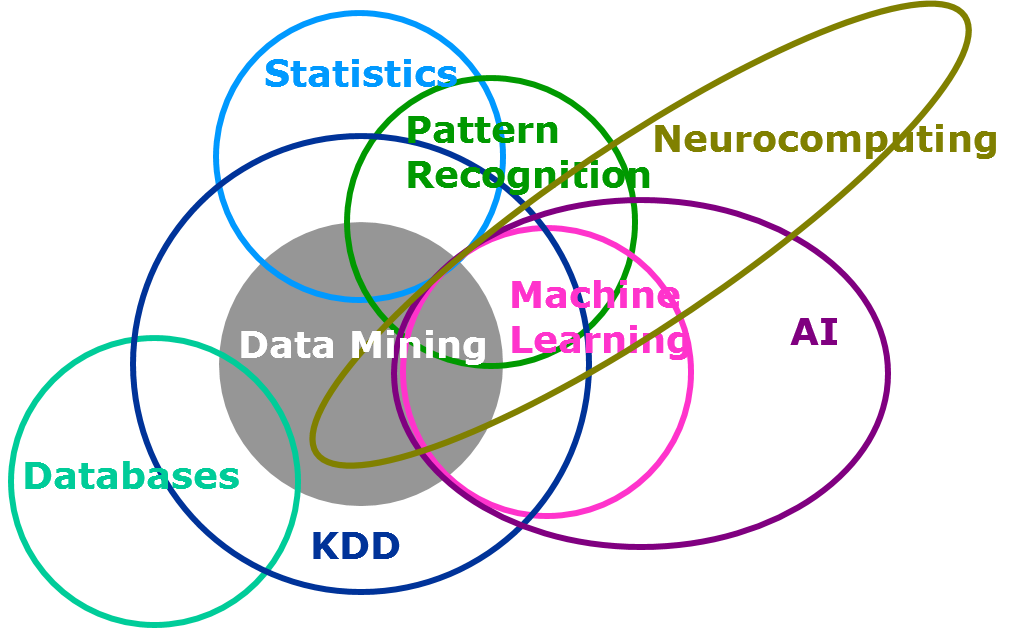
\includegraphics[width=0.8\linewidth]{data-mining-Venn-diagram}
\end{figure}
Image taken from: \hyperref[http://blogs.sas.com/content/subconsciousmusings/2014/08/22/looking-backwards-looking-forwards-sas-data-mining-and-machine-learning/]{''SAS, Data Mining and Machine Learning''}.
\end{frame}




\begin{frame}
\frametitle{What exactly is Machine Learning?}
\begin{figure}
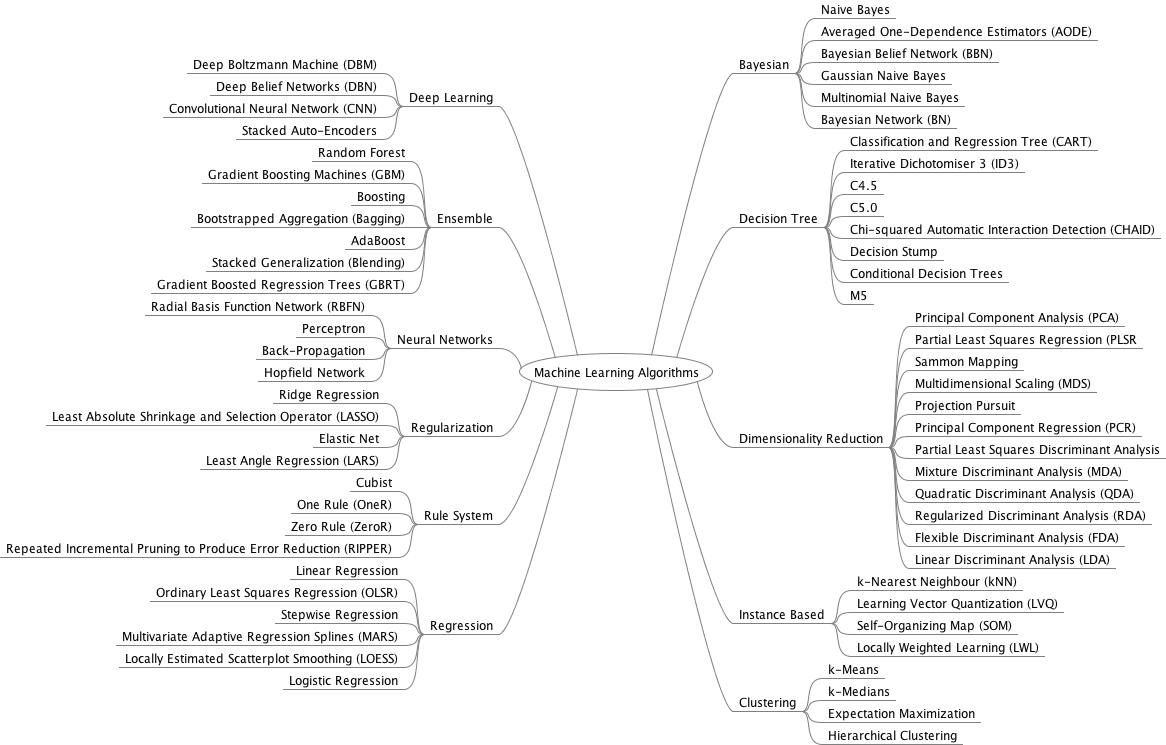
\includegraphics[width=0.9\linewidth]{MachineLearningAlgorithms}
\end{figure}
Image taken from: \hyperref[http://machinelearningmastery.com/a-tour-of-machine-learning-algorithms/]{''A Tour of Machine Learning Algorithms''}.
\end{frame}


%
%


%------------------------------------------------

\section{Multiple Kernel Learning}


\begin{frame}
\frametitle{MKL: meaning}

MKL:

"set of machine learning methods that use a predefined set of kernels and learn an optimal linear or non-linear combination of kernels as part of the algorithm"

\end{frame}



\begin{frame}
\frametitle{MKL: use in SVM}

SVM:

"given labeled training data (supervised learning), the algorithm outputs an optimal hyperplane which categorizes new examples"

\end{frame}


%set of machine learning methods that use a predefined set of kernels and learn an optimal linear or non-linear combination of kernels as part of the algorithm

\begin{frame}
\frametitle{MKL: use in SVM}

\begin{figure}
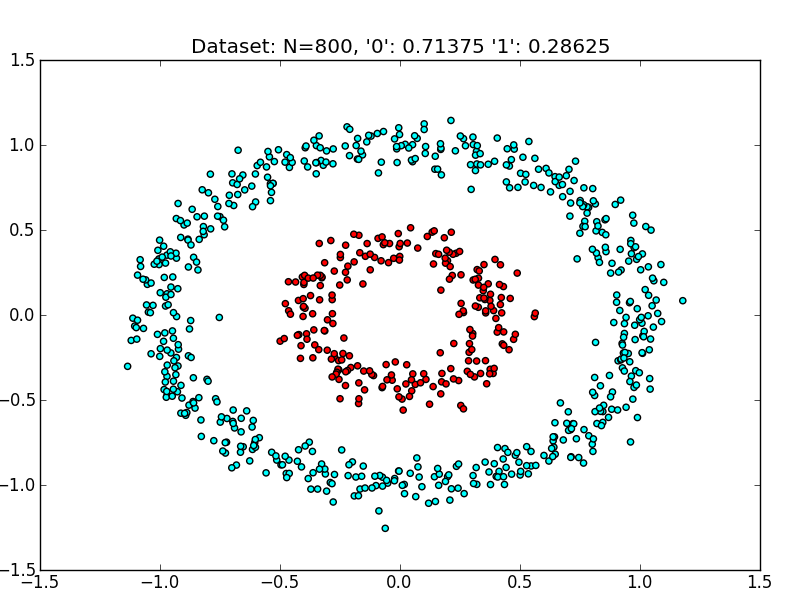
\includegraphics[width=0.9\linewidth]{dataset_nonsep}
\end{figure}
Image taken from: \hyperref[http://www.eric-kim.net/eric-kim-net/posts/1/kernel_trick.html]{''The Kernel Trick''}.

\end{frame}


\begin{frame}
\frametitle{MKL: use in SVM}

The Kernel trick:

\begin{itemize}
\item many ML algorithms (e.g. SVM) use the data only through inner products.
\item e.g. the following matrix (\textbf{kernel matrix}) can be used in classification and regression:
\end{itemize}

\begin{equation}
 X=\begin{bmatrix}
  \vec{x_{1}} \\
  \vec{x_{2}} \\
  ...\\
  \vec{x_{n}}
 \end{bmatrix} \rightarrow 
  K = XX^{T}
\end{equation}

\end{frame}



\begin{frame}
\frametitle{MKL: use in SVM}

The Kernel trick:

\begin{itemize}
\item the idea is to apply a transformation $\phi(\vec{x})$, which preserves the form of $K$:
\end{itemize}

\[
K=
  \begin{bmatrix}
    \phi(\vec{x_{1}})^{T}\phi(\vec{x_{1}}) & \phi(\vec{x_{1}})^{T}\phi(\vec{x_{2}}) & ...  \\
    \phi(\vec{x_{2}})^{T}\phi(\vec{x_{1}}) & ... & ...  \\
    ... & ... & ...
  \end{bmatrix}
\]

\end{frame}


\begin{frame}
\frametitle{MKL: use in SVM}

The Kernel trick:

\begin{itemize}
\item simple example (on a $\phi$ preserving the form of $K$):

\begin{itemize}
\item transformation $\phi$: $(x_{1}, x_{2})\rightarrow (z_{1}, z_{2}, z_{3}) = (x_{1}^{2}, \sqrt{2}x_{1}x_{2}, x_{2}^{2})$
\item let's take: $\vec{r} = \phi(\vec{a})$ and $\vec{s} = \phi(\vec{b})$
\item $\Rightarrow (\vec{r}\cdot\vec{s})_{3D} = r_{1}s_{1}+r_{2}s_{2}+r_{3}s_{3} = (a_{1}^{2})(b_{1}^{2})+(\sqrt{2}a_{1}a_{2})(\sqrt{2}b_{1}b_{2})+(a_{2}^{2})(b_{2}^{2})$
\item $\Rightarrow (\vec{r}\cdot\vec{s})_{3D} = (\vec{a}\cdot\vec{b})^{2}$
\end{itemize}

\item then, the Kernel trick consists of only knowing how to compute the inner product in the new space (through a function of the inner product in the original space), but not the actual transformation
\end{itemize}

\end{frame}



\begin{frame}
\frametitle{MKL: the Kernel trick}

\begin{figure}
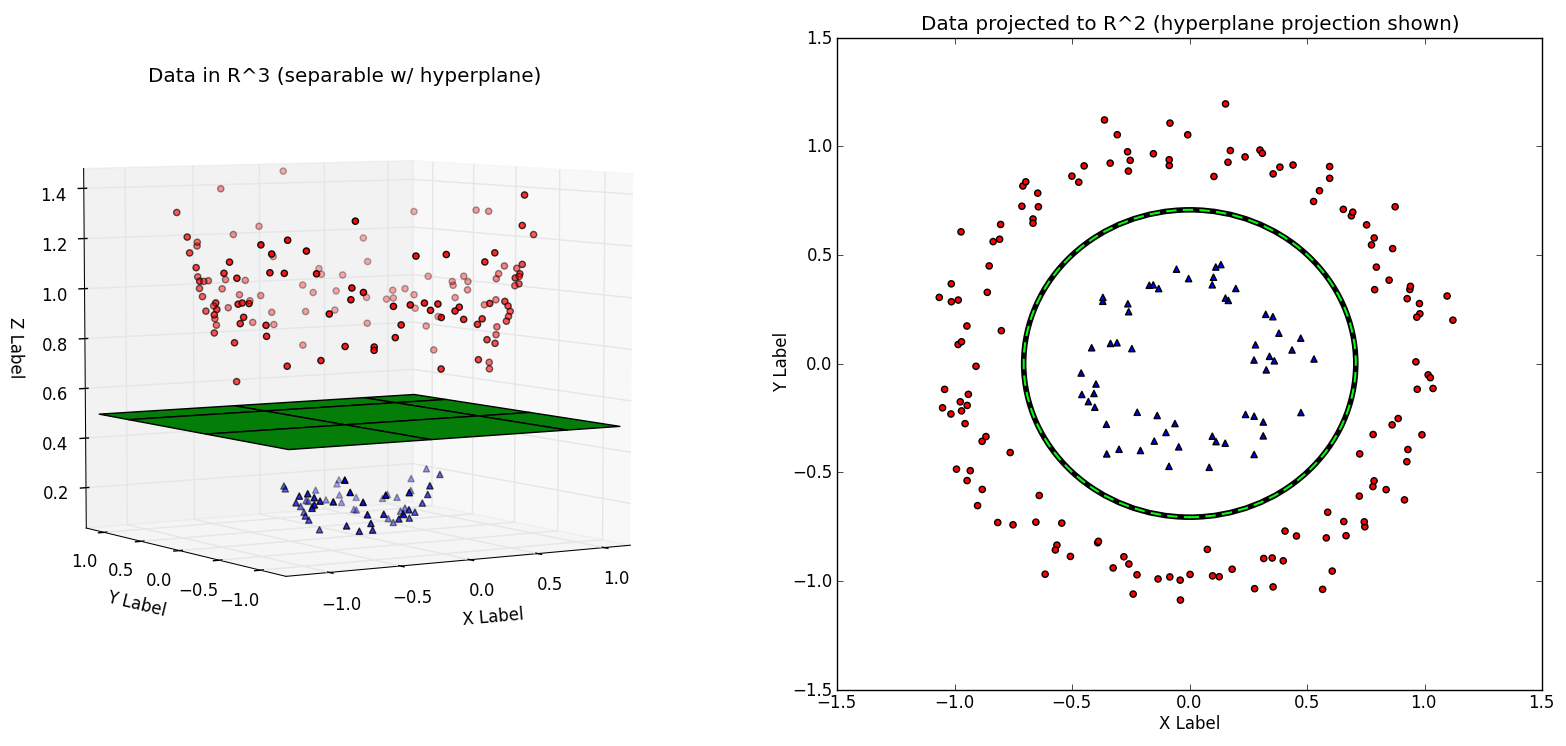
\includegraphics[width=1\linewidth]{data_2d_to_3d_hyperplane}
\end{figure}
Image taken from: \hyperref[http://www.eric-kim.net/eric-kim-net/posts/1/kernel_trick.html]{''The Kernel Trick''}.

\end{frame}



\begin{frame}
\frametitle{MKL: the Kernel trick}

MKL:

\begin{itemize}
\item extension of the Kernel trick, using many $\phi$'s now, and optimize with the original algorithm (SVM or other) but taking those kernels into account
\end{itemize}

\end{frame}




%------------------------------------------------

\begin{comment}

\section{Boosted Methods and Boosted Decision Trees}


\begin{frame}
\frametitle{BDT: decision trees}

\begin{figure}
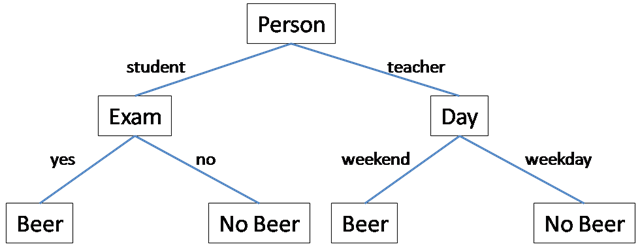
\includegraphics[width=1\linewidth]{detresb}
\end{figure}
Image taken from: \hyperref[https://computersciencesource.wordpress.com/2010/01/10/year-2-machine-learning-decision-trees/]{''Machine Learning - Decision Trees''}.


\end{frame}



\begin{frame}
\frametitle{BDT: boosted methods}

Explanation of Boosted methods.. and Boosted Decision Trees here..

\end{frame}


%IMPORTANT: restrictions on the application of the model.

%Supervised or unsupervised??

\end{comment}

%------------------------------------------------

\section{Applications}

\begin{frame}
\frametitle{Applications of ML}

Prediction in cancer:

\begin{figure}

\includegraphics[width=1\linewidth]{article_cancer}
\end{figure}

\end{frame}

\begin{frame}
\frametitle{Applications of ML}

Recommender systems (Netflix, Amazon, etc.), data mining, image recognition, etc.

\end{frame}


\begin{comment}
\begin{frame}
\frametitle{Applications of BDT}

Write here a couple of specific applications, particular to BDT...

\end{frame}
\end{comment}



%------------------------------------------------










%------------------------------------------------



\begin{comment}

\begin{frame}
\frametitle{Paragraphs of Text}
Sed iaculis dapibus gravida. Morbi sed tortor erat, nec interdum arcu. Sed id lorem lectus. Quisque viverra augue id sem ornare non aliquam nibh tristique. Aenean in ligula nisl. Nulla sed tellus ipsum. Donec vestibulum ligula non lorem vulputate fermentum accumsan neque mollis.\\~\\

Sed diam enim, sagittis nec condimentum sit amet, ullamcorper sit amet libero. Aliquam vel dui orci, a porta odio. Nullam id suscipit ipsum. Aenean lobortis commodo sem, ut commodo leo gravida vitae. Pellentesque vehicula ante iaculis arcu pretium rutrum eget sit amet purus. Integer ornare nulla quis neque ultrices lobortis. Vestibulum ultrices tincidunt libero, quis commodo erat ullamcorper id.
\end{frame}

%------------------------------------------------

\begin{frame}
\frametitle{Bullet Points}
\begin{itemize}
\item Lorem ipsum dolor sit amet, consectetur adipiscing elit
\item Aliquam blandit faucibus nisi, sit amet dapibus enim tempus eu
\item Nulla commodo, erat quis gravida posuere, elit lacus lobortis est, quis porttitor odio mauris at libero
\item Nam cursus est eget velit posuere pellentesque
\item Vestibulum faucibus velit a augue condimentum quis convallis nulla gravida
\end{itemize}
\end{frame}

%------------------------------------------------

\begin{frame}
\frametitle{Blocks of Highlighted Text}
\begin{block}{Block 1}
Lorem ipsum dolor sit amet, consectetur adipiscing elit. Integer lectus nisl, ultricies in feugiat rutrum, porttitor sit amet augue. Aliquam ut tortor mauris. Sed volutpat ante purus, quis accumsan dolor.
\end{block}

\begin{block}{Block 2}
Pellentesque sed tellus purus. Class aptent taciti sociosqu ad litora torquent per conubia nostra, per inceptos himenaeos. Vestibulum quis magna at risus dictum tempor eu vitae velit.
\end{block}

\begin{block}{Block 3}
Suspendisse tincidunt sagittis gravida. Curabitur condimentum, enim sed venenatis rutrum, ipsum neque consectetur orci, sed blandit justo nisi ac lacus.
\end{block}
\end{frame}

%------------------------------------------------

\begin{frame}
\frametitle{Multiple Columns}
\begin{columns}[c] % The "c" option specifies centered vertical alignment while the "t" option is used for top vertical alignment

\column{.45\textwidth} % Left column and width
\textbf{Heading}
\begin{enumerate}
\item Statement
\item Explanation
\item Example
\end{enumerate}

\column{.5\textwidth} % Right column and width
Lorem ipsum dolor sit amet, consectetur adipiscing elit. Integer lectus nisl, ultricies in feugiat rutrum, porttitor sit amet augue. Aliquam ut tortor mauris. Sed volutpat ante purus, quis accumsan dolor.

\end{columns}
\end{frame}

%------------------------------------------------
%\section{Second Section}
%------------------------------------------------

\begin{frame}
\frametitle{Table}
\begin{table}
\begin{tabular}{l l l}
\toprule
\textbf{Treatments} & \textbf{Response 1} & \textbf{Response 2}\\
\midrule
Treatment 1 & 0.0003262 & 0.562 \\
Treatment 2 & 0.0015681 & 0.910 \\
Treatment 3 & 0.0009271 & 0.296 \\
\bottomrule
\end{tabular}
\caption{Table caption}
\end{table}
\end{frame}

%------------------------------------------------

\begin{frame}
\frametitle{Theorem}
\begin{theorem}[Mass--energy equivalence]
$E = mc^2$
\end{theorem}
\end{frame}

%------------------------------------------------

\begin{frame}[fragile] % Need to use the fragile option when verbatim is used in the slide
\frametitle{Verbatim}
\begin{example}[Theorem Slide Code]
\begin{verbatim}
\begin{frame}
\frametitle{Theorem}
\begin{theorem}[Mass--energy equivalence]
$E = mc^2$
\end{theorem}
\end{frame}\end{verbatim}
\end{example}
\end{frame}

%------------------------------------------------

\begin{frame}
\frametitle{Figure}
Uncomment the code on this slide to include your own image from the same directory as the template .TeX file.
%\begin{figure}
%\includegraphics[width=0.8\linewidth]{test}
%\end{figure}
\end{frame}

%------------------------------------------------

\begin{frame}[fragile] % Need to use the fragile option when verbatim is used in the slide
\frametitle{Citation}
An example of the \verb|\cite| command to cite within the presentation:\\~

This statement requires citation \cite{p1}.
\end{frame}

\end{comment}

%------------------------------------------------

\begin{frame}
\frametitle{References}
\footnotesize{
\begin{thebibliography}{99} % Beamer does not support BibTeX so references must be inserted manually as below

%A community effort to assess and improve drug sensitivity prediction algorithms

\bibitem[Costello, 2006]{p1} James C Costello, \textit{et al.} (2014)
\newblock A community effort to assess and improve drug sensitivity prediction algorithms
\newblock \emph{Nature Biotechnology} 32, 1202–1212 %1531 -- 1565.

\bibitem[Sonnenburg, 2006]{p1} S{\"o}ren Sonnenburg, \textit{et al.} (2006)
\newblock Large Scale Multiple Kernel Learning
\newblock \emph{Journal of Machine Learning Research} 1531 -- 1565.


\end{thebibliography}
}
\end{frame}

%------------------------------------------------

\begin{frame}
\Huge{\centerline{The End}}
\end{frame}

%----------------------------------------------------------------------------------------

\end{document} 